\section{Flutter}
\setauthor{Antonio Kuvac}
Flutter ist ein Open-Source-Framework für die Entwicklung von mobilen Anwendungen, Webanwendungen und Desktop-Anwendungen. 
Es wurde von Google entwickelt und erstmals im Jahr 2017 veröffentlicht. 
Flutter verwendet die Programmiersprache Dart und eine eigene Widget-Bibliothek, um eine reaktionsfähige und ansprechende Benutzeroberfläche zu erstellen.

\subsection{Vorteile}
Flutter bietet mehrere Vorteile:

\begin{compactitem}
    \item \textbf{Plattformübergreifende Entwicklung}: Mit Flutter können Entwickler plattformübergreifende Anwendungen erstellen, die auf verschiedenen Betriebssystemen wie iOS, 
    Android, Web und Desktop laufen. Dies reduziert die Entwicklungskosten und spart Zeit und Ressourcen.
    \item \textbf{Schnelle Entwicklung}: Flutter bietet die Funktion "Hot Reload", die es Entwickler*innen ermöglicht, Änderungen in Echtzeit zu sehen, 
    ohne die Anwendung neu starten zu müssen. Dadurch wird die Entwicklung von Flutter-Anwendungen schneller und effizienter.
    \item \textbf{Reaktionsfähigkeit}: Flutter-Anwendungen sind schnell und reaktionsfähig, da sie auf der leistungsstarken Grafik-Engine Skia basieren. 
    Dies ermöglicht es Entwickler*innen, reibungslose Benutzererfahrungen mit flüssigen Animationen und Grafiken zu schaffen.
    \item \textbf{Einfache UI-Erstellung}: Mit der eigenen Widget-Bibliothek von Flutter können Entwickler*innen schnell und einfach ansprechende Benutzeroberflächen erstellen. 
    Die Bibliothek enthält viele vorgefertigte Widgets, die einfach angepasst werden können.
    \item \textbf{Native Performance}: Flutter-Anwendungen werden in nativem Code ausgeführt, was zu einer höheren Leistung und Geschwindigkeit führt als bei Hybrid- oder webbasierten Anwendungen.
\end{compactitem}

\subsection{Dart}

Dart ist die von Flutter verwendete Programmierspreche. Sie ist eine objektorientierte Programmiersprache, die von Google entwickelt wurde. Sie wurde erstmals im Jahr 2011 vorgestellt und ist eine relativ neue Programmiersprache im Vergleich zu anderen Sprachen wie Java, 
Python und C++. Die Sprache wurde entwickelt, um die Herausforderungen bei der Entwicklung von Webanwendungen zu bewältigen und ist auch für die Entwicklung von plattformübergreifenden mobilen Anwendungen geeignet.

Sie ist eine statisch typisierte Sprache, was bedeutet, dass Variablen und Funktionen vor der Laufzeit überprüft werden. Dadurch können Entwickler*innen Fehler frühzeitig erkennen und vermeiden.
Die Sprache unterstützt auch dynamische Typisierung, was die Entwicklung von Anwendungen erleichtert, die auf sich ändernden Datenstrukturen basieren.

Dart ist eine schnelle Sprache, die eine effiziente Ausführung ermöglicht und eine hohe Leistung bietet. Es ist auch eine einfach zu erlernende Sprache.

Dart bietet auch eine Vielzahl von Funktionen, die die Entwicklung von Anwendungen erleichtern. Dazu gehören Funktionen wie asynchrone Programmierung, 
um die Leistung bei der Verarbeitung von Netzwerk- und E/A-Operationen zu verbessern, sowie die Möglichkeit, Funktionen als Parameter zu übergeben, 
um die Flexibilität und Wiederverwendbarkeit von Code zu erhöhen.
\pagebreak
\section{Visual Studio Code}
\setauthor{Antonio Kuvac}
Visual Studio Code ist ein kostenloses, plattformübergreifendes Code-Editor-Tool von Microsoft. Es ist ein beliebtes Tool für Entwickler*innen, 
da es eine Vielzahl von Funktionen und Erweiterungen bietet, um die Produktivität und Effizienz zu verbessern.

Visual Studio Code bietet eine intuitive Benutzeroberfläche, die es Entwickler*innen erleichtert, schnell und einfach zu navigieren und Code zu schreiben. 
Es bietet auch integrierte Debugging-Tools, die Entwickler*innen helfen, Fehler zu finden und zu beheben, sowie integrierte Versionskontrolltools für Git, 
um Änderungen am Code effektiv zu verwalten.

\subsection{Extensions}
Eine der wesentlichsten Funktionen in VS Code sind Extensions (Erweiterungen). VS Code-Extensions können verschiedene Funktionen bieten, 
wie z.B. Syntax-Hervorhebung, Autovervollständigung, Debugging-Tools, Git-Integration und vieles mehr. 
Es gibt eine breite Palette von Erweiterungen, die für verschiedene Programmiersprachen und Frameworks verfügbar sind, 
um die Entwicklungserfahrung zu verbessern und die Produktivität zu steigern.

Die Installation von VS Code-Extensions ist einfach und unkompliziert. Sie können über den Visual Studio Code-Marktplatz oder direkt aus der Editor-Benutzeroberfläche installiert werden.
Nach der Installation stehen die neuen Funktionen und Tools sofort zur Verfügung.
\pagebreak
\section{Docker}
\setauthor{Antonio Kuvac}
Docker ist eine Open-Source-Plattform, die es Entwicklern ermöglicht, Anwendungen in isolierten Containern zu erstellen, bereitzustellen und auszuführen. 
Docker-Container sind leichtgewichtig und portabel und bieten eine effektive Möglichkeit, Anwendungen in verschiedenen Umgebungen und Infrastrukturen auszuführen.

\subsection{Funktionsweise}
Docker verwendet Container, um Anwendungen zu isolieren und eine konsistente Umgebung für ihre Ausführung zu schaffen. Container sind ähnlich wie virtuelle Maschinen, 
jedoch leichter und schneller zu erstellen, da sie den Kernel des Host-Betriebssystems nutzen. Jeder Container enthält alles, was eine Anwendung zum Ausführen benötigt, 
einschließlich des Codes, der Abhängigkeiten und der Konfiguration.

Die Funktionsweise von Docker basiert auf einem Schichtmodell, das aus drei Komponenten besteht:

\begin{enumerate}
    \item \textbf{Docker Engine}: Dies ist das Kernstück von Docker und besteht aus dem Docker-Daemon und der Docker-CLI (Command Line Interface). Der Docker-Daemon ist ein Hintergrundprozess, 
    der die Verwaltung und Ausführung von Containern übernimmt, während die Docker-CLI als Schnittstelle für den Benutzer dient, um mit dem Docker-Daemon zu interagieren.
    \item \textbf{Images}: Ein Docker-Image ist eine Vorlage oder Blaupause für die Erstellung von Containern. 
    Es enthält den Code, die Abhängigkeiten und Konfigurationen einer Anwendung sowie alle anderen erforderlichen Komponenten, die zur Ausführung der Anwendung benötigt werden. 
    Docker-Images werden über Docker Files erstellt, die eine Liste von Anweisungen enthalten, um das Image zu konfigurieren und zu erstellen.
    \item \textbf{Container}: Ein Docker-Container ist eine Instanz eines Docker-Images, die ausgeführt wird. Ein Container kann gestartet, gestoppt und gelöscht werden. 
    Jeder Container ist isoliert und hat seine eigene Dateisystemumgebung, Netzwerkschnittstellen und Ressourcenlimits.
    \end{enumerate}

    \begin{figure}[H]
        \centering
        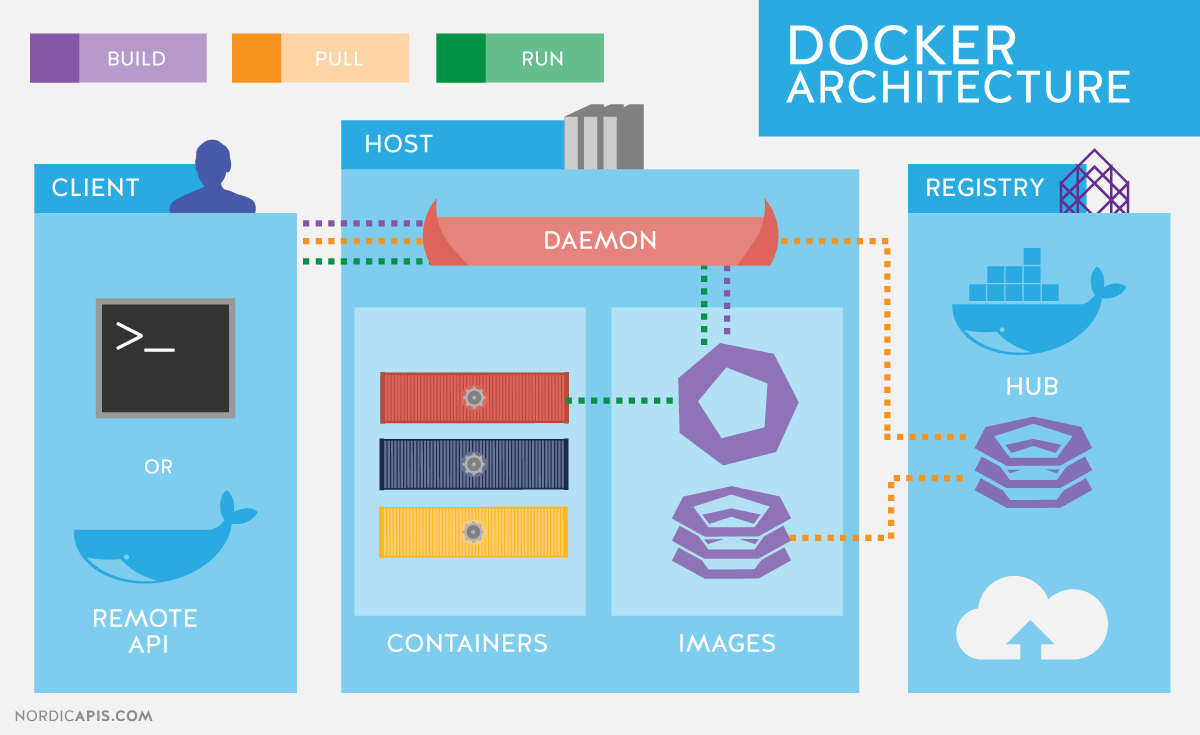
\includegraphics[scale=0.3]{pics/Docker_Architecture.png}
        \caption{Docker Architektur}
    \end{figure}

\subsection{Vorteile}
\begin{itemize}
    \item \textbf{Portabilität}: Docker-Container sind plattformunabhängig und können auf verschiedenen Betriebssystemen und Infrastrukturen ausgeführt werden.
    
    \item \textbf{Flexibilität}: Mit Docker können Anwendungen schnell erstellt, abgeändert und bereitgestellt werden, ohne die zugrunde liegende Infrastruktur ändern zu müssen.
    
    \item \textbf{Skalierbarkeit}: Docker ermöglicht eine einfache horizontale Skalierung von Anwendungen, indem es das Erstellen und Bereitstellen von Containern automatisiert.
    
    \item \textbf{Sicherheit}: Docker bietet Sicherheitsfunktionen wie Isolation und eingeschränkte Ressourcenkontrolle, um eine sicherere Ausführung von Anwendungen zu gewährleisten.
    
    \item \textbf{Effizienz}: Docker-Container sind leicht und benötigen weniger Ressourcen als virtuelle Maschinen, was zu einer höheren Effizienz und Leistung führt.
    \end{itemize}

    \section{Android Studio}
    \setauthor{Antonio Kuvac}
    Android Studio ist eine integrierte Entwicklungsumgebung (IDE), die speziell für die Entwicklung von Android-Apps entwickelt wurde. 
    Es wurde von Google entwickelt und ist kostenlos für Entwickler verfügbar, um Android-Apps zu erstellen und zu bearbeiten.

    \subsection{Funktionen}
    Android Studio verfügt über eine Vielzahl von Funktionen, die dabei helfen, schneller und effizienter Android-Apps zu entwickeln. Zu den wichtigsten Funktionen gehören:

    \begin{itemize}
        \item \textbf{Intelligentes Code-Editing:} Android Studio bietet intelligentes Code-Editing mit automatischen Vorschlägen, Fehlererkennung und Refactoring-Funktionen.
        \item \textbf{Emulator:} Entwickler können den Android-Emulator nutzen, um ihre Apps auf verschiedenen Android-Geräten zu testen, ohne physische Geräte besitzen zu müssen.
        \item \textbf{Layout-Editor:} Android Studio verfügt über einen Layout-Editor, mit dem Entwickler die Benutzeroberfläche ihrer Apps visuell gestalten können.
        \item \textbf{Gradle Build-System:} Android Studio verwendet das Gradle Build-System, das Entwicklern ermöglicht, komplexe Abhängigkeiten und Builds zu verwalten.
        \item \textbf{Integration mit anderen Tools:} Android Studio ist nahtlos in andere Google-Tools wie Firebase und Google Cloud Platform integriert.
        \end{itemize}

    \subsection{Emulator}
    Der Android Studio Emulator ist ein wichtiges Tool für Android-Entwickler, das es ihnen ermöglicht, ihre Apps auf verschiedenen Android-Geräten zu testen, ohne physische Geräte besitzen zu müssen. Der Emulator wird mit Android Studio mitgeliefert und kann einfach über die IDE gestartet werden.

Einer der größten Vorteile des Emulators ist, dass Entwickler ihre Apps auf verschiedenen Android-Versionen und Gerätekonfigurationen testen können, um sicherzustellen, 
dass ihre Apps auf allen unterstützten Geräten reibungslos funktionieren. 
Der Emulator kann eine Vielzahl von Android-Versionen und -Gerätekonfigurationen emulieren, einschließlich verschiedener Bildschirmauflösungen und -größen, 
Prozessortypen und Speicherkapazitäten.

Ein weiterer Vorteil des Emulators ist, dass er den Entwicklungsprozess beschleunigen kann, indem er den Build- und Bereitstellungsprozess verkürzt. 
Anstatt jedes Mal eine neue Version der App auf einem physischen Gerät zu testen, können Entwickler die App einfach im Emulator starten und testen, 
was Zeit spart und die Entwicklungszeit verkürzt.

Die Einrichtung des Emulators in Android Studio ist einfach und erfordert nur wenige Schritte. Entwickler müssen zunächst sicherstellen, 
dass sie die neueste Version von Android Studio heruntergeladen und installiert haben. Sobald sie Android Studio geöffnet haben, können sie den Emulator über das AVD Manager-Tool starten, 
das im Menü "Werkzeuge" zu finden ist.

Es gibt jedoch auch einige Nachteile beim Verwenden des Emulators. Einer der größten Nachteile ist die Geschwindigkeit. Da der Emulator ein virtuelles Gerät ist, 
kann er langsamer sein als ein physisches Gerät. Dies kann dazu führen, dass Entwickler länger warten müssen, um ihre Apps im Emulator zu testen.

Ein weiterer Nachteil ist, dass der Emulator nicht alle Funktionen eines physischen Geräts emulieren kann. Beispielsweise kann der Emulator keine Anrufe oder Textnachrichten empfangen und senden, 
da er kein physisches Mobilfunkmodem hat. Dies bedeutet, dass Entwickler nicht alle Aspekte ihrer App im Emulator testen können und gegebenenfalls auf physische Geräte zurückgreifen müssen.

Zusammenfassend lässt sich sagen, dass der Android Studio Emulator ein wertvolles Tool für Android-Entwickler ist, um ihre Apps auf verschiedenen Geräten und Android-Versionen zu testen. 
Obwohl der Emulator einige Nachteile hat, überwiegen die Vorteile in den meisten Fällen und er ist ein unverzichtbares Werkzeug für die App-Entwicklung.

\begin{figure}[H]
    \centering
    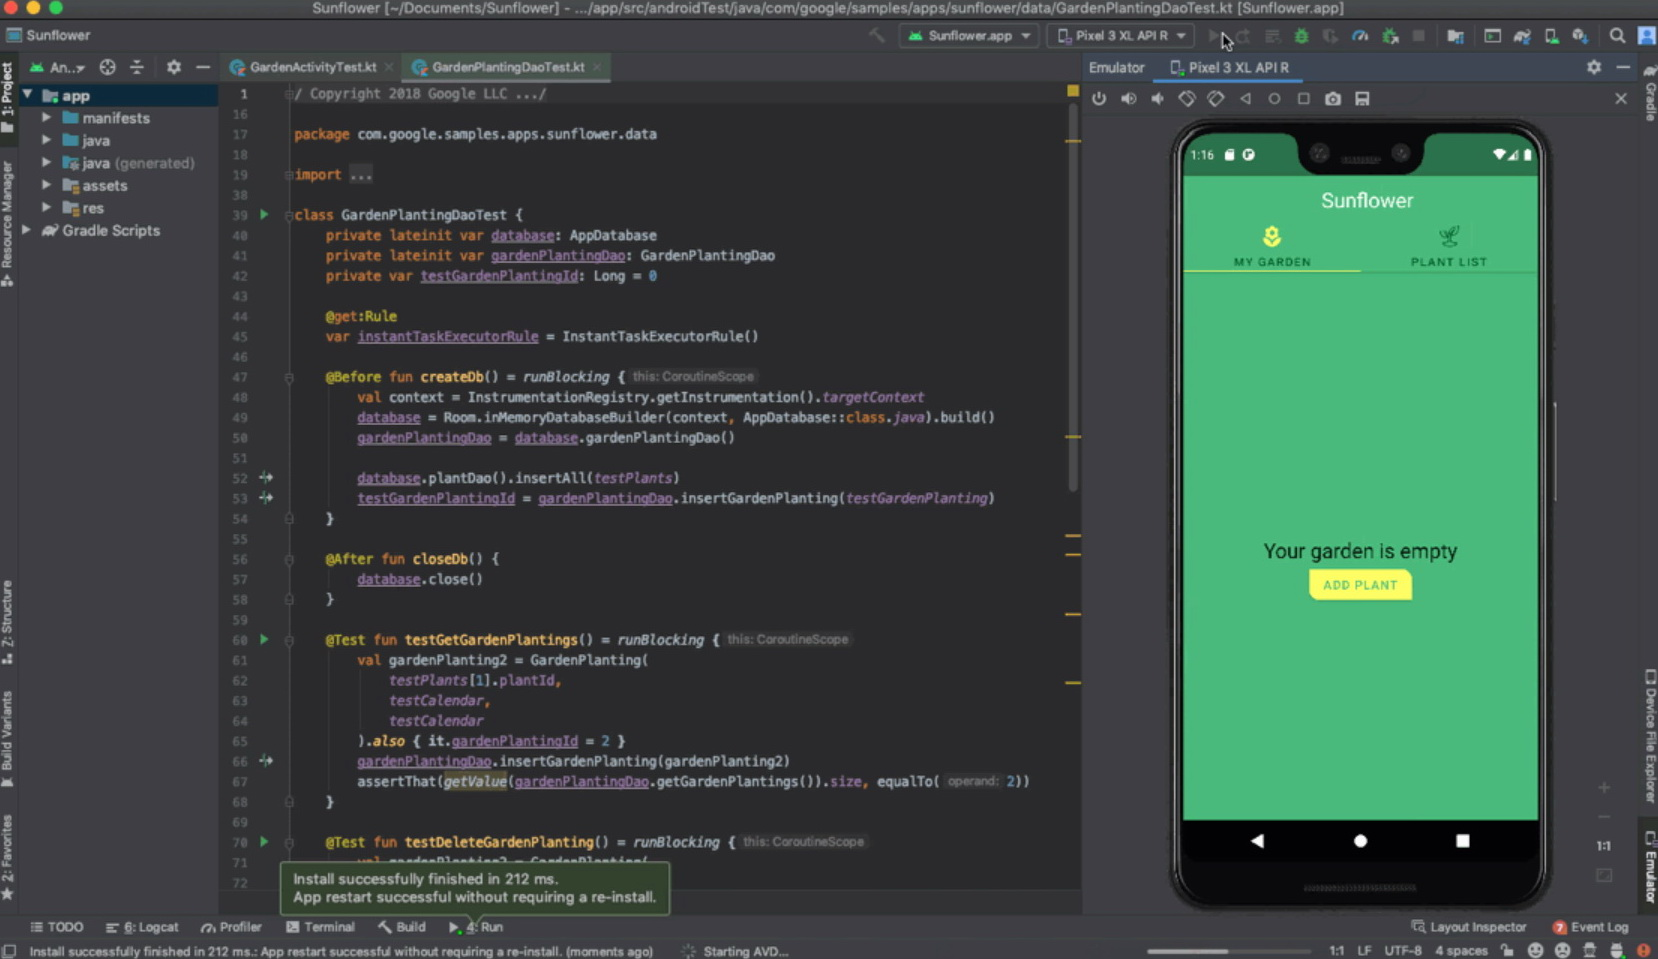
\includegraphics[scale=0.2]{pics/android-studio-emulator.jpg}
    \caption{Android Studio Emulator}
\end{figure}

\section{AdobeXD}
    \setauthor{Antonio Kuvac}

    AdobeXD ist eine Design-Software, die speziell für die Erstellung von Benutzeroberflächen und Interaktionen für Mobile Apps, Webseiten und andere digitale Plattformen entwickelt wurde.

\subsection*{Funktionen}
Die wichtigsten Funktionen sind intuitive Layout-Tools, um Entwürfe schnell zu erstellen und zu bearbeiten, Vektor-Tools, um hochwertige Grafiken zu erstellen, Prototyping-Funktionen, um interaktive Prototypen zu erstellen und zu testen und die Möglichkeit, Designs in Echtzeit zu teilen und Feedback von Stakeholdern zu erhalten.

\subsection*{Plattformübergreifendes Design} 
AdobeXD unterstützt plattformübergreifendes Design, was bedeutet, dass man nur eine einzige Design-Datei erstellen muss, um diese dann auf AdobeXD auf verschiedenen Geräten und Plattformen verwenden zu können. 
Das ermöglicht, schnell und effizient Designs für verschiedene Geräte und Plattformen zu erstellen.

\subsection*{Integration mit anderen Tools} 
AdobeXD ist nahtlos in andere Adobe-Tools wie Photoshop und Illustrator integriert. Das ermöglicht, Designs nahtlos zwischen verschiedenen Adobe-Tools zu übertragen. 
Es ist auch in andere Tools wie Slack und Microsoft Teams integriert, um die Zusammenarbeit zu erleichtern.

\subsection*{Cloud-basierte Zusammenarbeit} 
AdobeXD bietet eine Cloud-basierte Zusammenarbeit an, mit der es möglich ist, Designs in Echtzeit zu teilen und Feedback von Stakeholdern zu erhalten. 
Designer*innen können Links zu ihren Designs freigeben und Stakeholder können Kommentare und Feedback direkt in die Designs geben.

\section{IntelliJ}
\setauthor{Antonio Kuvac}

\textbf{IntelliJ} ist eine integrierte Entwicklungsumgebung (IDE) für die Softwareentwicklung, die von JetBrains entwickelt wurde. Die IDE ist in Java geschrieben und unterstützt eine Vielzahl von Programmiersprachen wie Java, Kotlin, Groovy, Scala, PHP, Python, und mehr. IntelliJ ist in zwei Versionen erhältlich: die Community Edition, die kostenlos erhältlich ist, und die Ultimate Edition, die kostenpflichtig ist und zusätzliche Funktionen und Tools bietet.

\subsection{Funktionen}

IntelliJ bietet zahlreiche Funktionen und Tools, um Entwicklern bei der Entwicklung von Softwareprojekten zu helfen. Hier sind einige der wichtigsten Funktionen:

\begin{itemize}
\item Code-Editing: IntelliJ bietet intelligentes Code-Editing mit Code-Vervollständigung, Syntax-Hervorhebung, Refactoring und Code-Analyse-Funktionen.
\item Debugger: Der integrierte Debugger ermöglicht es Entwicklern, Code zu debuggen und Fehler schnell zu finden.
\item Build-Tools: IntelliJ unterstützt eine Vielzahl von Build-Tools wie Gradle, Maven und Ant.
\item Integration mit anderen Tools: IntelliJ ist nahtlos in andere Tools und Frameworks wie Git, JUnit und Spring integriert.
\item Version-Control-System: IntelliJ unterstützt verschiedene Version-Control-Systeme wie Git, Subversion und Mercurial.
\item Code-Qualität: IntelliJ bietet Code-Qualität-Tools, um Entwicklern dabei zu helfen, fehlerfreien Code zu schreiben und Code-Qualitätsstandards einzuhalten.
\item Frameworks: IntelliJ unterstützt eine Vielzahl von Frameworks wie Spring, Hibernate, Struts und mehr.
\end{itemize}
\pagebreak

\subsection{Vorteile}

IntelliJ bietet eine Vielzahl von Vorteilen für Entwickler, darunter:

\begin{itemize}
\item Effizienz: IntelliJ verbessert die Effizienz der Entwickler durch seine intelligenten Funktionen und Tools.
\item Einfache Integration: IntelliJ lässt sich einfach in andere Tools und Frameworks integrieren.
\item Bessere Code-Qualität: Die Code-Qualität-Tools von IntelliJ helfen Entwicklern, fehlerfreien Code zu schreiben und Code-Qualitätsstandards einzuhalten.
\item Unterstützung verschiedener Programmiersprachen: IntelliJ unterstützt eine Vielzahl von Programmiersprachen und Frameworks.
\item Gute Dokumentation: Die Dokumentation von IntelliJ ist umfassend und hilft Entwicklern, die IDE schnell zu erlernen.
\end{itemize}